\section{Implementation} \label{sec:implementation}
\subsection{Registers} \label{sec:implementation:registers}
This section elucidates the intricate facets concerning the register-module implementation. It delves into the architectural nuances encompassing the driver module, data-pointer register, data structures, stack functionality, loop-skip mechanisms, instruction parsing, instruction-pointer management, and the flag register. By the conclusion of this chapter, a comprehensive overview integrating these components will be presented, encapsulating the holistic framework of the register-module.

\subsubsection{Overview}
Within the BFCPU framework, the ALU was intentionally omitted due to the constrained mathematical operations inherent in brainfck language, limited to singular addition and subtraction by one. To streamline complexity, our approach involved the utilization of 74LS193 and 74LS161 integrated chips, enabling the creation of discrete registers. These chips offer both memory storage capabilities and the ability to increment values. Moreover, the 74LS193 chip encompasses the added functionality of decrementing stored values, although such functionality remains unnecessary for the F-R component. Hence, the choice of 74LS** was deliberate, selected for its singular provision of 4-bit value storage, aligning precisely with the requirements of the system.

\subsubsection{Common INC-DEC functionality problem}
The Register module's intricate configuration involves numerous INC and DEC pins, necessitating manipulation by the control unit to modify register values. To streamline and unify this process, the Driver module acts as a centralized interface for all registers within the entire register-module structure. The fundamental concept underlying the Driver module revolves around consolidating multiple INC and DEC pins into a single pair, accompanied by a CLK (clock) input.

When both INC and DEC signals maintain identical voltage states (either low or high), the selected register operates in a mode referred to as "none" during the rising edge of the CLK. This signifies that the register's value remains unchanged—neither incremented nor decremented. Conversely, when the digital value of the INC-DEC pair registers as 01 or 10, the corresponding selected register experiences either an increment or a decrement in its value.

The output generated by the Driver module, in the form of the UP-DOWN signal pair, directs the appropriate action to the designated register. Notably, for registers utilizing the 74LS161 chip that exclusively permits incrementing, only an UP signal is necessary.

To facilitate register selection, a selecting interface is imperative to designate the specific register under manipulation. The inner circuitry (refer to figure \ref{fig:registerModuleOverview}) adeptly fulfills this function. The accompanying figure provides a broad overview of the register-module, showcasing the existence of three select pins capable of establishing eight distinct paths. This suffices, given the presence of fewer than eight unique registers within the system's architecture.

\begin{figure}[H]
	\centering
	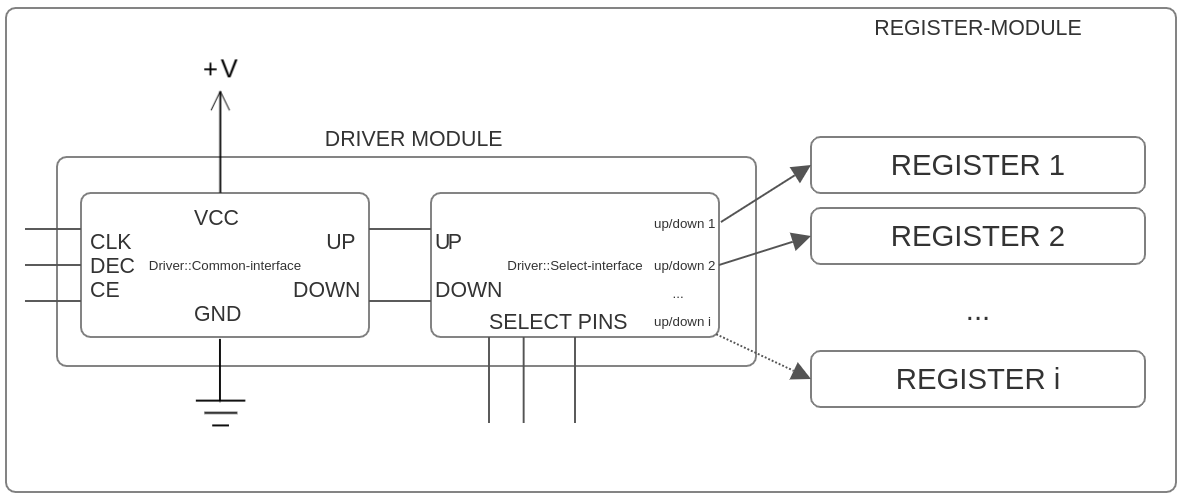
\includegraphics[width=0.9\textwidth]{img/register_module_overview}
	\caption{Register-module Overview}
	\label{fig:registerModuleOverview}
\end{figure}

\subsubsection{74LS193 Chaining}
The utilization of 74LS193 (or 74LS161) chips in the construction of registers provides both storage capacity and INC-DEC functionality. However, a singular 74LS193 chip inherently provides storage for 4 bits, which falls short of the 8 or 16 bits necessary for the registers' intended functionality. Fortunately, the 74LS193 chip offers a chaining capability, mitigating this limitation.

Through a chaining configuration wherein the Carry-Out (CO) of one chip connects to the Up (UP) pin of another, and the Borrow Out (BO) links to the Down (DOWN) pin, an expansion of available bits becomes feasible (refer to figure \ref{fig:registerModuleChaining}). This method effectively extends the storage capacity, enabling the aggregation of multiple chips to accommodate the required bit sizes. This chaining technique stands as a foundational element implemented across registers demanding more than 4 bits, ensuring their requisite storage depth and functionality.

\begin{figure}[H]
	\centering
	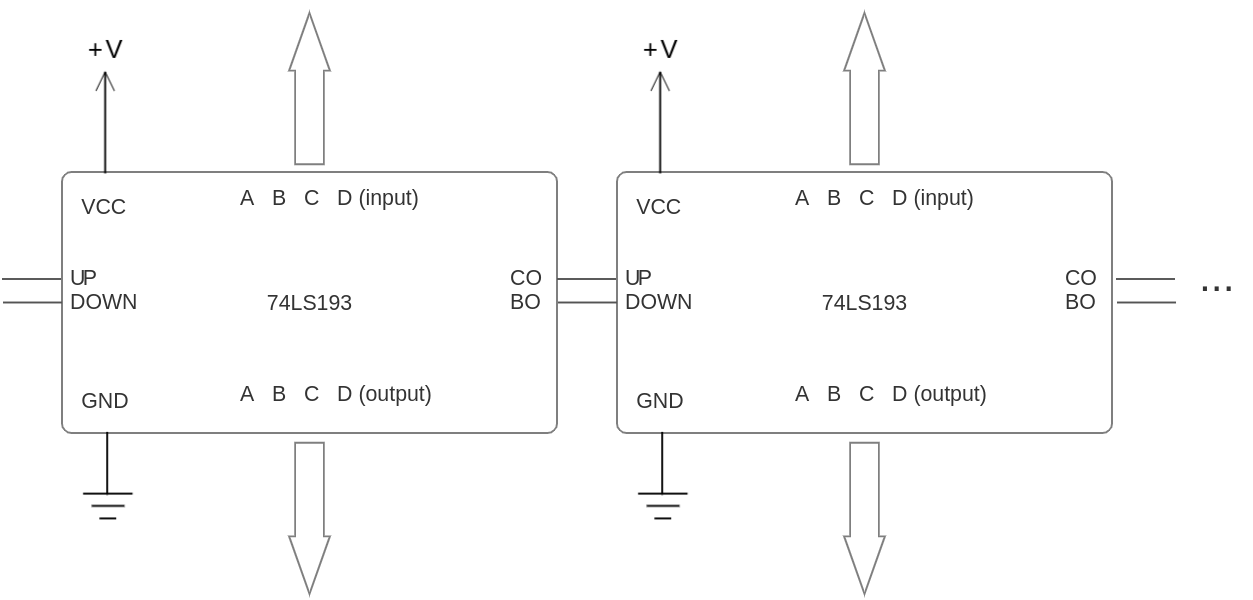
\includegraphics[width=0.9\textwidth]{img/register_module_chaining}
	\caption{Register-module 74LS193 chaining}
	\label{fig:registerModuleChaining}
\end{figure}

\subsubsection{Circuit: Driver Module}

In the computer's initial design phase, various concepts were explored for implementing this module. Initially, the demux-circuit was incorporated; however, it exhibited partial functionality, encountering persistent issues such as potential propagation delays and compatibility concerns with the 74LS193 chip. Resolving these issues in a sustainable and efficient manner posed considerable challenges.

Consequently, the decision was made to discard the initial driver module design (refer to Appendix A(\ref{sec:appendix:old_driver_module_design}) for an in-depth exploration of the former circuitry) in favor of developing an alternative circuit. This revised circuit now stands as the official and integral component of the computer's architecture, addressing the shortcomings and inefficiencies encountered in the prior design iteration.

The concept underlying the development of this stable driver module is rather straightforward:
\begin{itemize}
	\item Configure UP-DOWN\footnote{The output of the driver module} to a HIGH state when both INC and DEC signals are either high or low simultaneously.
	\item Generate a pulse on the UP signal while maintaining the DOWN signal high when INC is high and DEC is low.
	\item Generate a pulse on the DOWN signal while maintaining the UP signal high when INC is low and DEC is high.
\end{itemize}

The practical implementation details are visually represented in Figure \ref{fig:actual_driver_module_implementation}, accompanied by the following corresponding solutions:

\begin{itemize}
	\item Common Interface:
	\begin{itemize}
		\item Utilize $$CLK + (INC \oplus DEC)$$ to prevent pulsing when INC and DEC have identical values.
		\item Connect the resultant signal with the inverted INC-DEC into a NAND gate to ensure favorable behavior when INC and DEC have different values.
		\item Integration of additional inverters is imperative to ensure compatibility with both the registers and the select interface\footnote{The 3-to-8 demultiplexer used inverts the output}.
	\end{itemize}
	\item Select Interface:
	\begin{itemize}
		\item Establish connection of the UP-DOWN pair to the 3-to-8 demultiplexer, facilitating the routing of this pair to the input of the selected register.
	\end{itemize}
\end{itemize}


\begin{figure}[H]
	\centering
	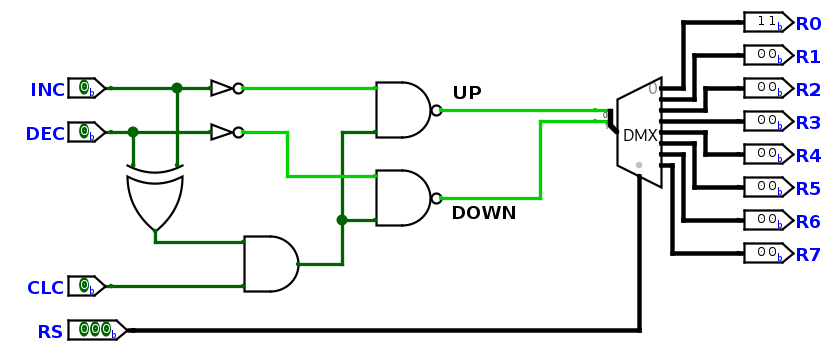
\includegraphics[width=0.9\textwidth]{img/actual_driver_module_implementation}
	\caption{The Actual Driver Module Implementation}
	\label{fig:actual_driver_module_implementation}
\end{figure}



\subsubsection{Circuit: Data Register}
The data register functions as an 8-bit valued flip-flop, equipped with both increment and decrement functionalities, which led to the adoption of the 74LS193 chip. An integral feature of the data register is its generation of a zero flag (Z), indicating a value of 1 exclusively when the stored value within the register is 0. The implementation of this particular feature involves the use of OR gates and direct connections to the stored bits (refer to Figure \ref{fig:dataRegisterImplementation} for a visual representation).


\begin{figure}[H]
	\centering
	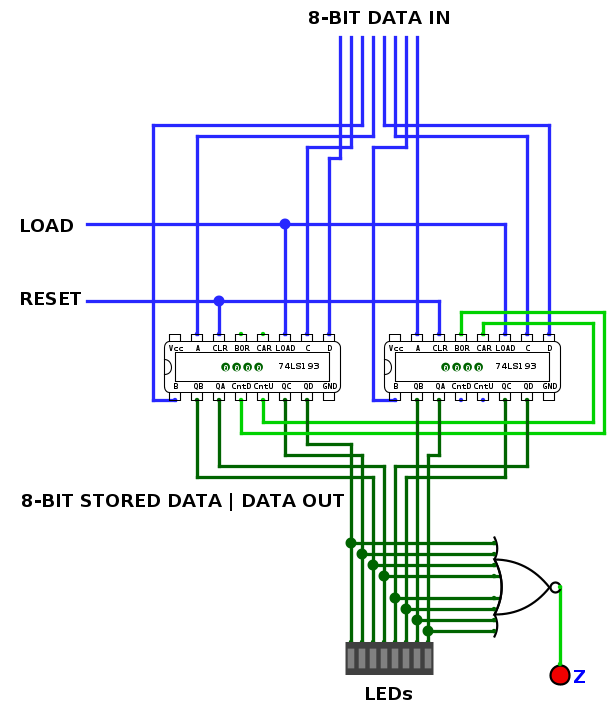
\includegraphics[width=0.9\textwidth]{img/data_register_implementation}
	\caption{Data, and Loop-Skip Register Implementation (\ref{sec:implementation:registers:loop_skip})}
	\label{fig:dataRegisterImplementation}
\end{figure}


\subsubsection{Circuit: Data-Pointer Register}
The Data-Pointer register operates as a 16-bit valued flip-flop equipped with both increment and decrement functionalities, consequently utilizing the 74LS193 chip. While the Data-Pointer register itself holds no distinct exceptional properties, its output (the stored value) maintains a connection to the bus transceiver, a characteristic shared among other registers as well\footnote{The implementation of the bus transceiver involves a straightforward approach: connecting only outputs alongside the DIR and CE (chip enable) pins as inputs, employing the 74LS245 chips}. Refer to Figure \ref{fig:dataPointerRegisterImplementation} for an illustrative depiction of its implementation.


\begin{figure}[H]
	\centering
	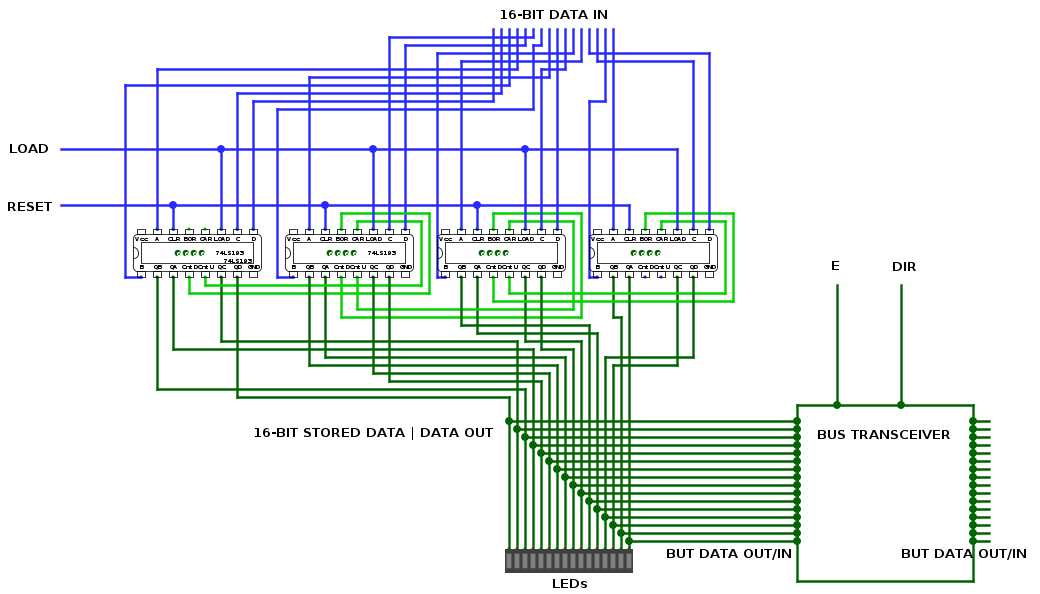
\includegraphics[width=0.9\textwidth]{img/data_pointer_register_implementation}
	\caption{Data-Pointer Register Implementation}
	\label{fig:dataPointerRegisterImplementation}
\end{figure}

\subsubsection{Circuit: Loop-Skip Register} \label{sec:implementation:registers:loop_skip}
At its core circuitry, the loop-skip register (LS-R) shares an identical implementation with the data register (D-R): both possess an 8-bit storage capacity, facilitate increment and decrement operations, and include a loop-flag functionality\footnote{The loop-flag mirrors the zero-flag in the data register, thus is implemented in a similar fashion as in the data register}. For an illustration of this implementation, please refer to Figure \ref{fig:dataRegisterImplementation}.


\subsubsection{Circuit: Instruction Register} \label{sec:implementation:registers:instruction}
As stated above for Loop-Skip Registers, the instruction register shares an identical implementation with the data register: both possess an 8-bit storage capacity. However, an internal circuitry contains 74LS**** chips instead of 74LS193. The underlying reason is derived from unnecessary decrement functionality \footnote{Instruction Register stores current operation machine code, which can only be loaded from the ROM}. We will dive deeper in \ref{sec:control_unit}.

\subsubsection{Circuit: Instruction-Pointer Register}
The instruction-pointer register (IP-R) shares its implementation framework with the data-pointer register. However, as the IP-R specifically denotes the machine code's location stored in the ROM, its sole requirement is for increment functionality. The procedural nature of brainf*ck dictates sequential code processing. Consequently, rather than utilizing the 74LS193, the choice fell upon the 74LS161 chip for its capacity to exclusively handle increments.

\subsubsection{Circuit: Flag Register}
The Flag Register is designed to manage precisely two bits, functioning as a 2-bit latch. Notably, our available inventory comprises chips configured for 4-bit operations, hence, two additional bits within the Flag Register remain reserved for potential future modifications. For this purpose, the LS74**** chip was selected to serve as the Flag Register. (!!!!!!!!!!!!! WHAT CHIP WE USE)


\subsection{Memory} \label{sec:implementation:memory}


\subsection{Control Unit} \label{sec:implementation:control_unity}


\subsection{Input} \label{sec:implementation:input}


\subsection{Output} \label{sec:implementation:output}

